\subsection{Análises cinemática, dinâmica e
controle do manipulador}

A análise da simulação revela as áreas da pá que podem ser revestidas,
as áreas de mais difícil acesso, e as posições da base do manipulador para a
execução bem sucedida da operação, levando em consideração a cinemática,
dinâmica e controle do manipulador. 

A metodologia percorre os seguintes tópicos: 1) discretização da pá; 2)
avaliação de revestimento dos extremos da pá, restringindo a base a um trilho
idealizado pelo projeto mecânico; 3) teste de revestimento completo; 4) teste de
revestimento de áreas até então não revestidas, sugerindo novas posições para a
base. Onde 1) já foi previamente avaliado em \textit{EMMA-DETAIL}. 

As variáveis do processo de revestimento são: 1) pistola de revestimento
é aproximada por um cilindro de 300 mm de comprimento e 50 mm de raio, 
acoplada à extremidade do efetuador; 2) as pás da turbina podem girar em seu
próprio eixo de $0^o$ a $29^o$; 3) o rotor da turbina pode girar de
$0^o$ a $360^o$; 4) a distância entre extremidade da pistola e pá deve
ser mantida em $235 \pm 5$ mm durante toda a operação; 4) o ângulo entre a
pistola e o plano da pá deve ser $90^o \pm 60^o$, mas é aconselhável uma
tolerância máxima de $30^o$.

Além disso, vale observar algumas conclusões feitas no relatório
\textit{EMMA-DETAIL}: 1) a análise cinemática verifica se, dado um ponto da
pá, há alguma configuração das juntas para revestí-lo; 2) a análise dinâmica
mostrou que, durante a execução de uma trajetória, se o manipulador estiver
muito próximo do ponto que deseja revestir, os ângulos das juntas tendem a
variar muito, aumentando drasticamente os torques e impossibilitando a operação.


\subsubsection{Avaliação dos extremos da pá} 

É fácil observar que as áreas de mais difícil acesso à pá são suas extremidades,
áreas em preto da figura~\ref{fig::extremidades}, devido ao alcance do robô e
por serem áreas em que a pá apresenta maior inclinação. A alteração da direção
do vetor normal à pá e a posição do ponto a ser revestido são os fatores 
importantes para a aplicação de revestimento, isto é, pontos em uma posição
elevada para o robô e vetor normal direcionada para cima são complexos. Observe
a figura~\ref{fig::normal}, o vetor $\vec{P}$ é um exemplo de vetor normal
pertencente a um ponto da pá de difícil revestimento, tanto pela posição quanto
pelo vetor normal.

\begin{figure}[!ht]
	\centering	
	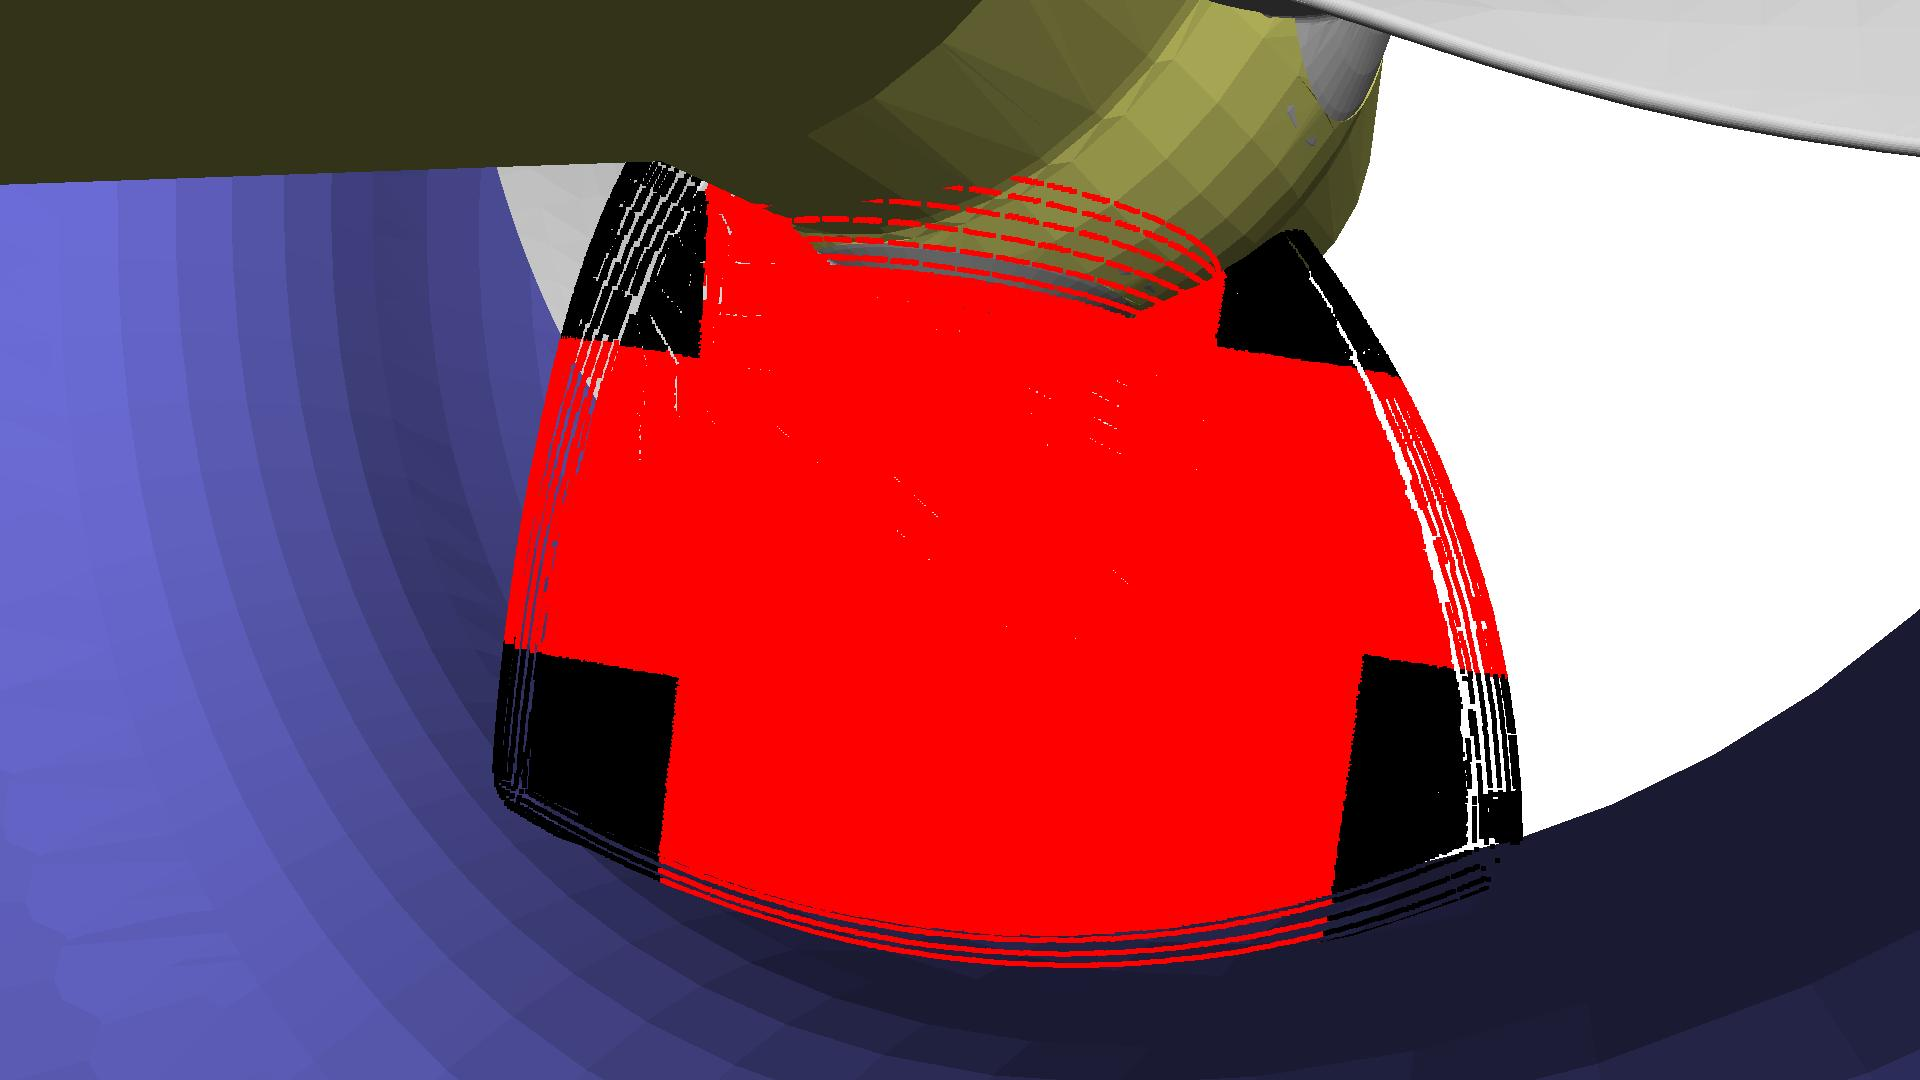
\includegraphics[width=0.9\columnwidth]{method/figs/tocoat.jpg}
	\caption{Extremidades da pá em preto.}
	\label{fig::extremidades}
\end{figure}

\begin{figure}[!ht]
	\centering	
	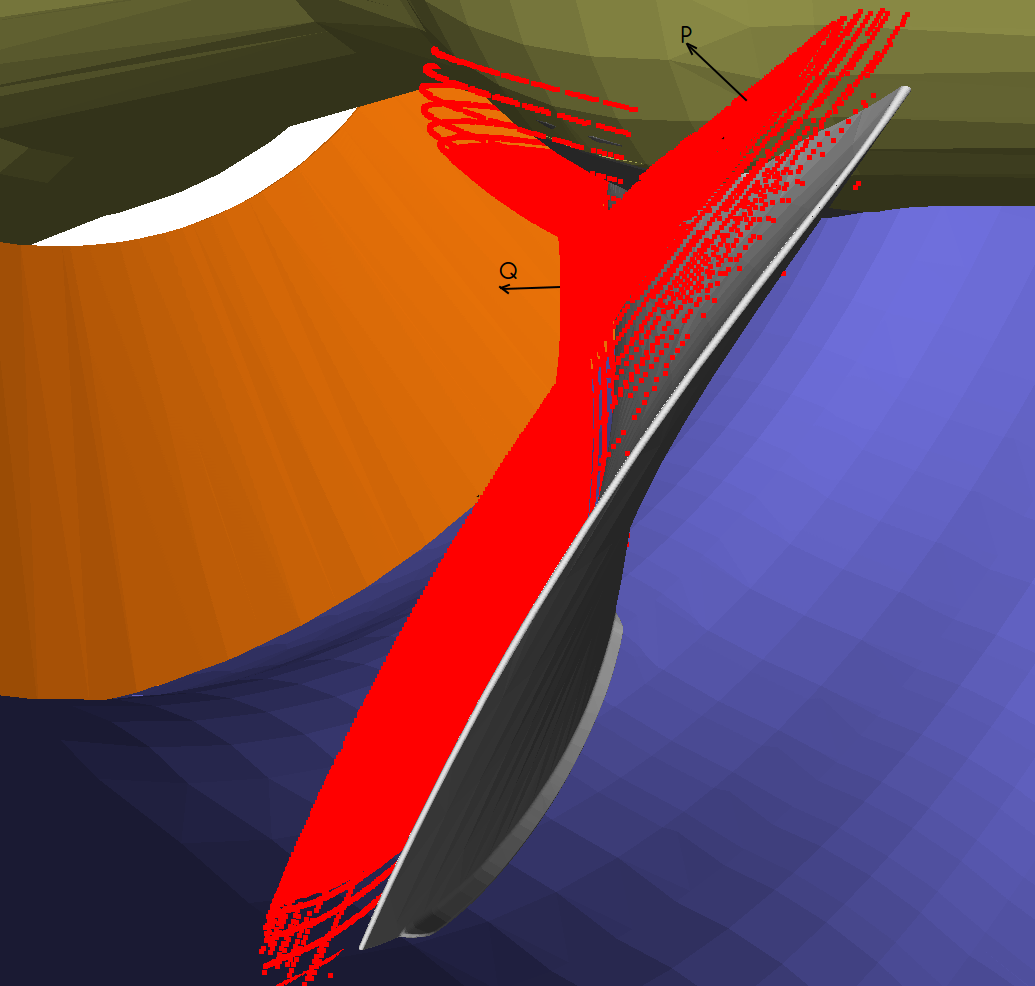
\includegraphics[width=0.9\columnwidth]{method/figs/normal.png}
	\caption{Vetores normais (em preto) de pontos a serem revestidos (em
	vermelho).}
	\label{fig::normal}
\end{figure}

A simulação de teste de revestimento das extremidades considerou as seguintes
variáveis: 1) os ângulos das pás da turbina foram fixados em $24^o$, ângulo
natural de uso; 2) avaliou-se o giro do rotor de $0^o$ a $30^o$ com passo de
$3^o$; 3) a distância entre extremidade da pistola e pá pode variar $235 \pm 5$
mm; 4) o ângulo entre a pistola e o plano da pá pode variar $90^o \pm 30^o$; 5)
a posição em $y$ do robô pode variar $-2970 \pm 250$ mm (posição global) com
passo de 50 mm; 6) a posição em $x$ do robô pode variar $715 \pm 485$ mm em
relação à pá com passo de 50 mm; 7) a posição em $z$ do robô foi amostrada
uniformemente em 7 pontos ao longo da pá.

A figura~\ref{fig::trilho2all} mostra todas as posições simuladas para a base do
robô. As restrições dessas posições são a altura mínima da base ao aro câmara e
a altura do robô. Para cada posição de base e ângulo do rotor, foi simulado o
processo de revestimento para as quatro extremidades da pá, levando em
consideração as respectivas tolerâncias.

\begin{figure}[!ht]
	\centering	
	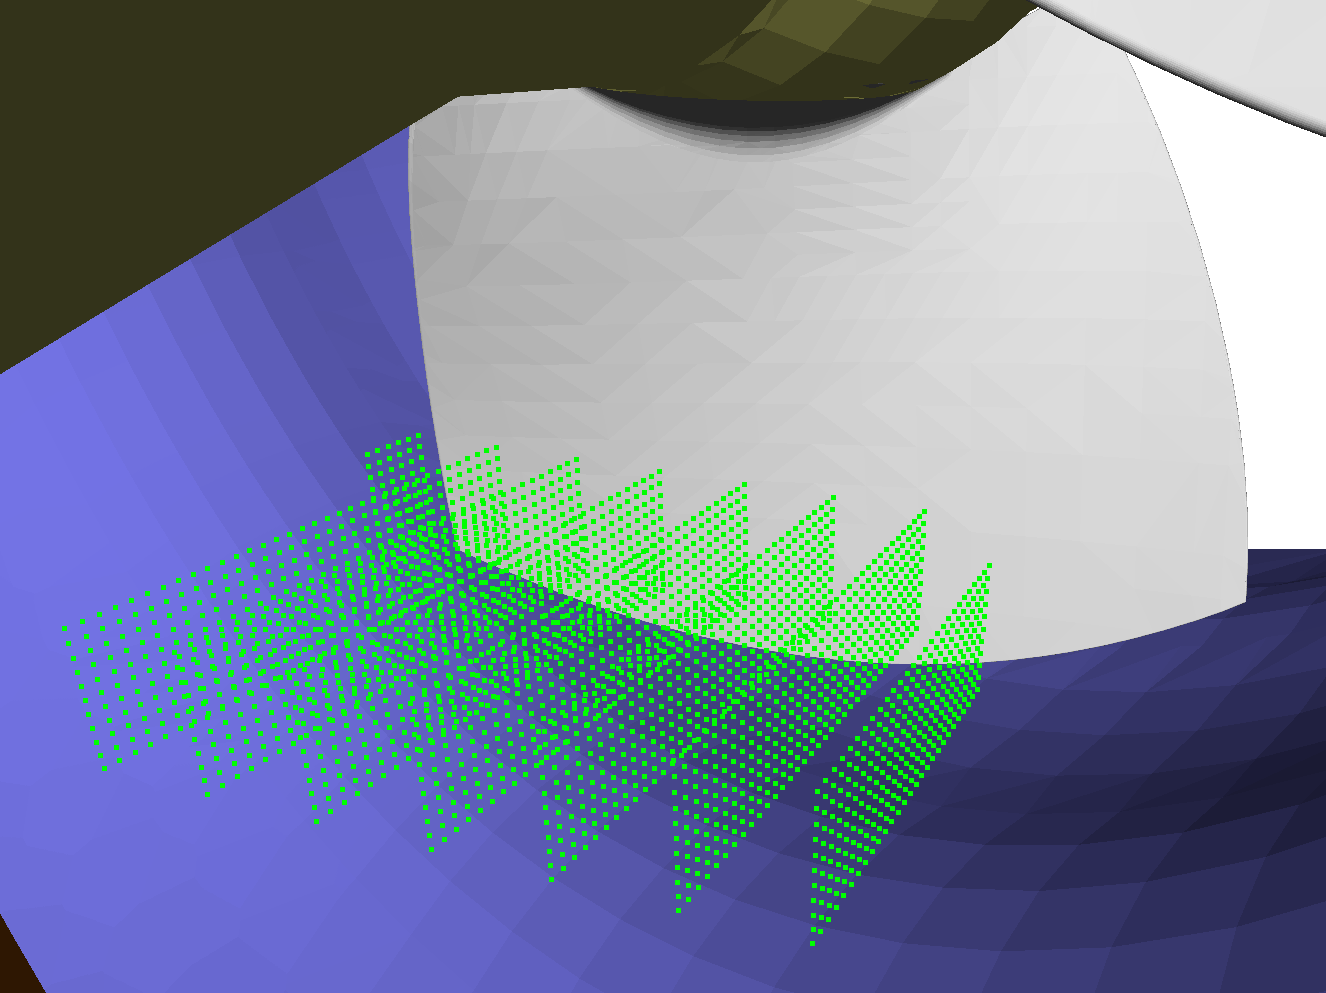
\includegraphics[width=\columnwidth]{method/figs/trilho2all.png}
	\caption{Possíveis posições da base do robô, em verde.}
	\label{fig::trilho2all}
\end{figure}

Nas subseções seguintes, serão analisadas cada extremidade da
pá independentemente, considerando as varíaveis acima.

\paragraph{Extremidade inferior esquerda}

A extremidade inferior esquerda apresenta a complexidade de posição do ponto a
ser revestido, visto que os pontos estão na borda, próximas ao aro câmara,
aumentando o risco de colisões. A figura~\ref{fig::footleft} mostra a
discretização da pá na extremidade esquerda: pontos azuis são pontos revestidos
na tolerância de $30^o$; em preto, pontos revestidos sem tolerância; e em
vermelho, pontos que não foram revestidos para esta posição do robô.

\begin{figure}[!ht]
	\centering	
	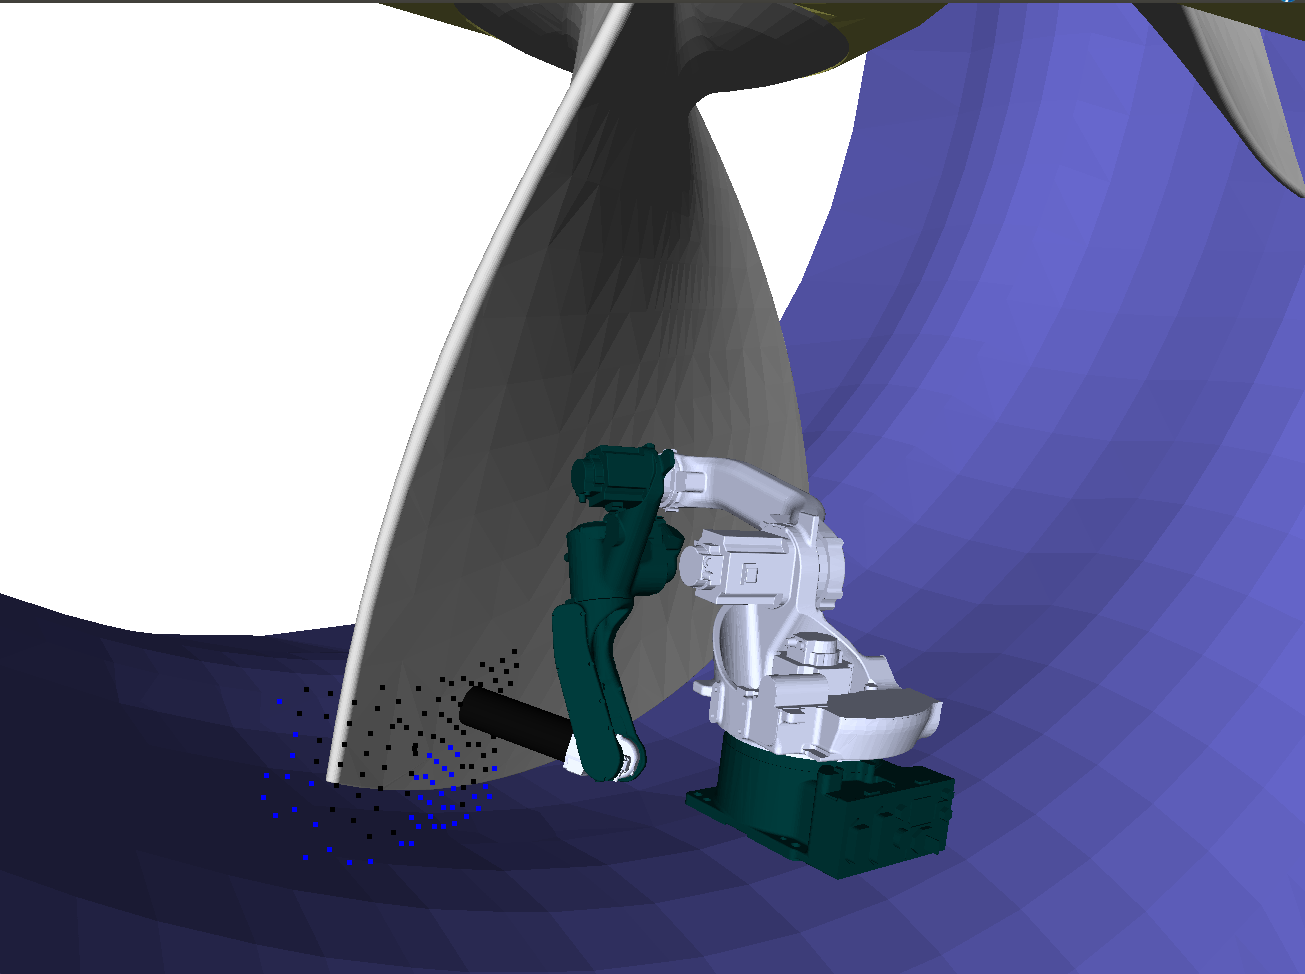
\includegraphics[width=\columnwidth]{method/figs/footleft.png}
	\caption{Estudo de revestimento para a extremidade inferior esquerda.}
	\label{fig::footleft}
\end{figure}

A simulação mostrou que o robô foi capaz de revestir toda a extremidade, na
altura mínima $y=-3220$ mm, a uma distância de até $x=1200$ mm da pá. Conforme o
robô se aproxima da pá, verifica-se que a altura pode sofrer variações
positivas, por exemplo para $x=980$ mm, $y=-3070$ mm. Entretanto, como já foi
verificado na simulação dinâmica, não é aconselhável aproximar o robô da pá a
uma distância inferior a $x=1000$ mm, pois os torques durante a execução podem ser
elevados.

Dessa forma, a extremidade inferior esquerda não mostrou desafios técnicos.

\paragraph{Extremidade inferior direita}

A extremidade inferior direita possui complexidade de posição do ponto a
ser revestido maior que a extremidade inferior esquerda, visto que a extremidade
está mais próxima da área em que a curvatura do aro é superior a $20^o$ (base
mais próxima do solo). A figura~\ref{fig::footright} mostra a discretização da
pá na extremidade esquerda: pontos azuis são pontos revestidos na tolerância de
$30^o$; em preto, pontos revestidos sem tolerância; e em vermelho, pontos que
não foram revestidos para esta posição do robô.

\begin{figure}[!ht]
	\centering	
	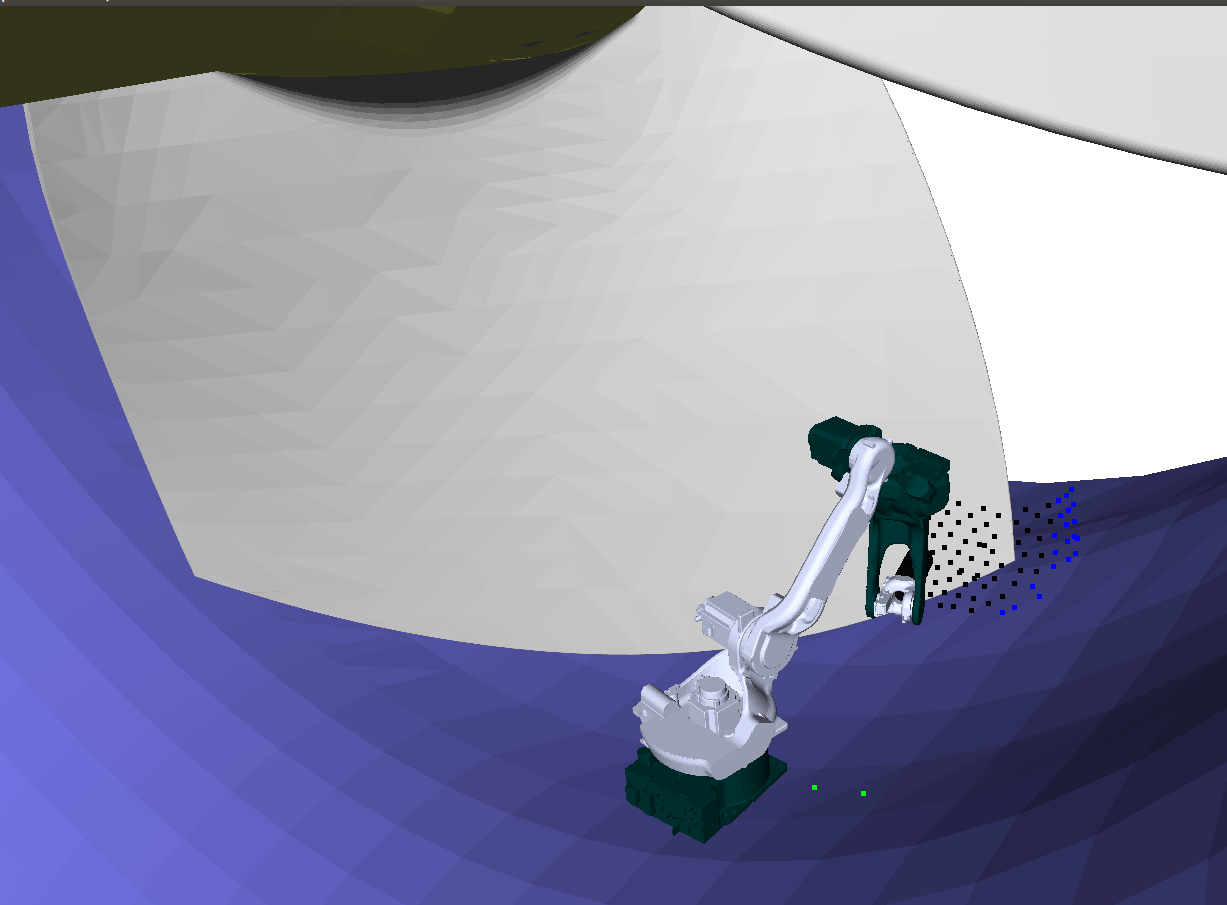
\includegraphics[width=\columnwidth]{method/figs/footright.png}
	\caption{Estudo de revestimento para a extremidade inferior direita.}
	\label{fig::footright}
\end{figure}

A simulação mostrou que o robô foi capaz de revestir toda a extremidade, na
altura mínima $y=-3220$ mm, a uma distância de até $x=1200$ mm da pá. 

Dessa forma, a extremidade inferior direita não mostrou desafios técnicos.

\paragraph{Extremidade superior esquerda}\label{superioresquerda}

A extremidade superior esquerda possui complexidade de posição do ponto a
ser revestido devido à altura do robô. A figura~\ref{fig::shoulderleft} mostra
a discretização da pá na extremidade esquerda: pontos azuis são pontos revestidos na tolerância de
$30^o$; em preto, pontos revestidos sem tolerância; e em vermelho, pontos que
não foram revestidos para esta posição do robô.

\begin{figure}[!ht]
	\centering	
	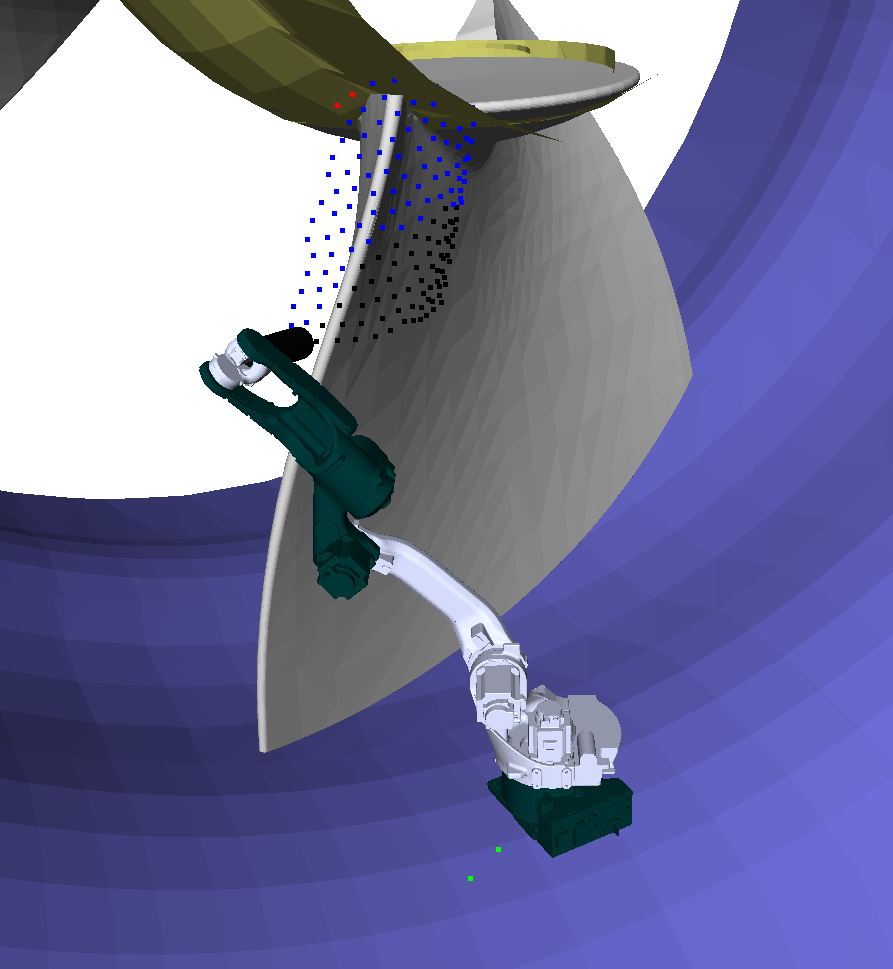
\includegraphics[width=\columnwidth]{method/figs/shoulderleft.png}
	\caption{Estudo de revestimento para a extremidade superior esquerda.}
	\label{fig::shoulderleft}
\end{figure}

A simulação mostrou que se mantivermos a altura da base em $y=-3220$ mm
(altura mínima) e $x=1200$ mm, são necessárias duas posições em $z$ (ao longo do
trilho) para o revestimento completo da extremidade. É interessante para o
projeto manter altura fixa o quanto possível, pois há redução de grau de
liberdade, e, portanto, redução na complexidade da base mecânica.

Caso haja alteração na altura do robô, por exemplo  $y=-2770$ mm, só será
necessária uma posição em $z$ para a conertura completa da região. Mas é
preferível mover o robô no trilho, em $z$, a mover o robô em altura, em $y$. 

A extremidade superior esquerda necessitou duas posições para a base, mas não
mostrou desafios técnicos.

\paragraph{Extremidade superior direita}

A extremidade superior esquerda possui duas complexidades de revestimento:
posição do ponto devido à altura do robô; e vetor normal, direção de
revestimento. A figura~\ref{fig::shoulderright} mostra a discretização da pá na
extremidade esquerda: pontos azuis são pontos revestidos na tolerância de $30^o$; em preto, pontos revestidos sem tolerância; e em vermelho, pontos que
não foram revestidos para esta posição do robô.

\begin{figure}[!ht]
	\centering	
	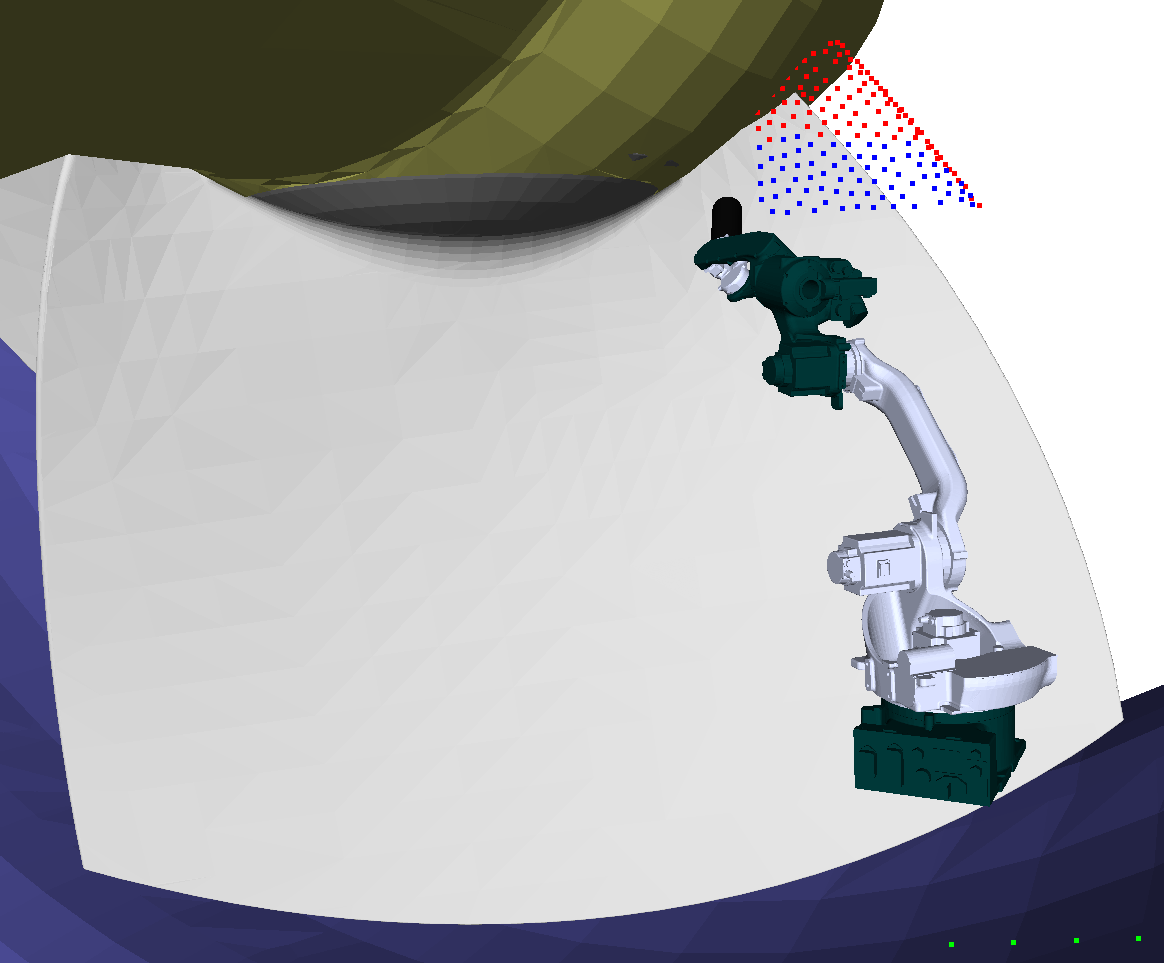
\includegraphics[width=\columnwidth]{method/figs/shoulderright.png}
	\caption{Estudo de revestimento para a extremidade superior direita.}
	\label{fig::shoulderright}
\end{figure}

A simulação mostra que, mesmo se utilizarmos a altura máxima para a base
$y=-2720$ mm e mantivermos $x=1200$ mm, não há posição em $z$ (ao longo do
trilho) para revestir por completo a extremidade. Aproximando o manipulador da
pá, novos pontos são revestido, mas mesmo em $x=230$ mm o
revestimento não é completo. O mesmo teste foi feito para diferentes
ângulos do rotor, mas os resultados não são favoráveis, pois conforme o rotor
gira, a pá se afasta do robô.

Para $y=-3220$ mm e $x=1200$ mm, nenhum ponto da extremidade superior direita é
revestido, logo outras estratégias devem ser adotadas. A extremidade superior
direita mostrou grande complexidade técnica e não foi possível encontrar uma
solução viável para o 2º trilho a fim de revestí-la.

\paragraph{Conclusão da simulação de extremidades}

Os resultados da simulação das extremidades da pá mostraram que três das
quatro extremidades da pá podem ser revestidas sem problemas técnicos, e
mantendo fixas as variáveis $y=-3220$ mm (referência global) e $x=1200$ mm de
distância em relação à pá. A extremidade superior direita ainda não apresenta
solução de revestimento utilizando o trilho 2 com as tolerâncias especificadas.

A rotação da turbina também foi simulada de $0^o$ a $30^o$. Entretanto, como
em $0^o$ as três extremidades foram revestidas sem alteração de dois graus de
liberdade $x$ e $y$, escolheu-se manter o rotor em $0^o$ para esta aplicação.

\subsubsection{Teste de revestimento completo e novas soluções de base}

Após a avaliação das extremidades da pá, deve-se ainda simular o revestimento
total, pois a superfície da pá é muito irregular, podendo se aproximar ou se
afastar do robô para certas posições de base. Além disso, foram abordadas novas
estratégias para a solução de revestimento da extremidade direita da pá. A
simulação de teste de toda a pá considerou as seguintes variáveis:

\begin{itemize}
  \item O ângulo de ataque das pás da turbina variam de $0^o$ a $29^o$. 
  O acréscimo deste
  grau de liberdade buscou solucionar o problema da extremidade direita.
  \item O rotor da turbina foi girado de $0^o$ a $30^o$ com passo de $3^o$.
  Manteve-se este grau de liberdade, pois em conjunto com o giro da pá, o
  problema da extremidade superior direita poderia ser solucionado.
  \item A distância entre extremidade da pistola e pá pode variar $235
  \pm 5$ mm.
  \item O ângulo entre a pistola e o plano da pá pode variar $90^o \pm
  30^o$. Alguns testes utilizaram a tolerância limite de $60^o$ como tentativa
  de revestir a extremidade direita superior.
  \item A posição em $y$ do robô foi mantida fixa. $-3220$ mm na referência
  global.
  \item A posição em $x$ do robô foi mantida fixa. $1200$ mm de
  distância em relação a pá.
  \item A posição em $z$ do robô foi amostrada uniformemente em 10 pontos ao
  longo da pá. A equipe de mecânica restringiu o movimento em $z$ tal que
  $-1240 < z < 1240$, garantindo para este $y$ mínimo ($-3220$ mm) espaço
  suficiente para a construção do trilho.
\end{itemize}

A restrição da mecânica para a construção do trilho $-1240$ mm $< z <$ $1240$ mm
prejudica o revestimento na lateral direita da pá, região em que o aro câmara
está próximo de $20^o$. A figura~\ref{fig::simcomp1_1} mostra a
discretização completa da pá, nas condições em que o rotor está $0^o$ e a pá
$24^o$:
em preto, pontos revestidos; e em vermelho, pontos que não foram revestidos. As
figuras seguintes adotarão a mesma legenda de cores para os pontos revestidos.
Como pode ser visto, não foi possível revestir os pontos da lateral direita, a extremidade superior direita e a extremidade superior esquerda.

\begin{figure}[!ht]
	\centering	
	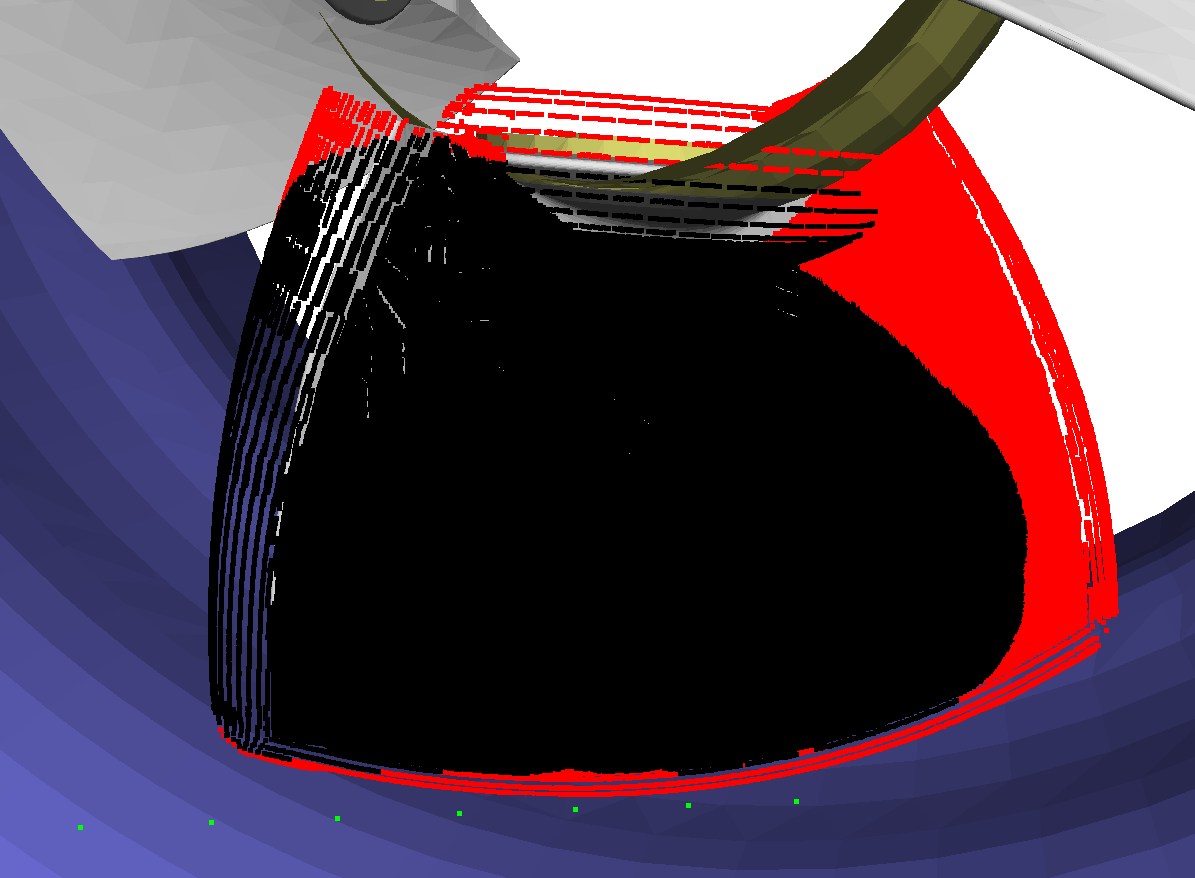
\includegraphics[width=\columnwidth]{method/figs/simcomp1_1.png}
	\caption{Simulação de revestimento completo da pá, considerando as
	restrições mecânicas da base, ângulo $0^o$ do rotor e $24^o$ da pá.}
	\label{fig::simcomp1_1}
\end{figure}

\paragraph{Extremidade superior esquerda}
Há três possíveis soluções para revestir a extremidade superior esquerda:
elevação da base do robô; aumentar tolerância de ângulo de revestimento para
$60^o$; e rotação da turbina para $-15^o$. Como esta
região da pá tem inclinação projetada para o robô, alterar o ângulo da pá de $24^o$ para $0^o$ não favorece o
revestimento (figura~\ref{fig::simcomp1_4}). Em termos de operação, as três
medidas possuem desvantagens: rotacionar a turbina é complexo, visto que será
necessário realizar um procedimento para transportar os equipamentos a uma área
de segurança e fazer a recalibração; elevar o robô apresenta complexidade
mecânica, já que exige mais um grau de liberdade da base, e fazer recalibração;
aumentar a tolerância do ângulo de revestimento tem complexidade menor, mas
aumenta a perda de material de revestimento.

A figura~\ref{fig::simcomp1_5} mostra a discretização completa da pá, nas
condições em que o rotor está $-15^o$ e a pá $24^o$. Conforme o rotor é
girado no sentido horário (negativo), o revestimento na extremidade superior
esquerda da pá é completa, porém o lado direito fica prejudicado.

\begin{figure}[!ht]
	\centering	
	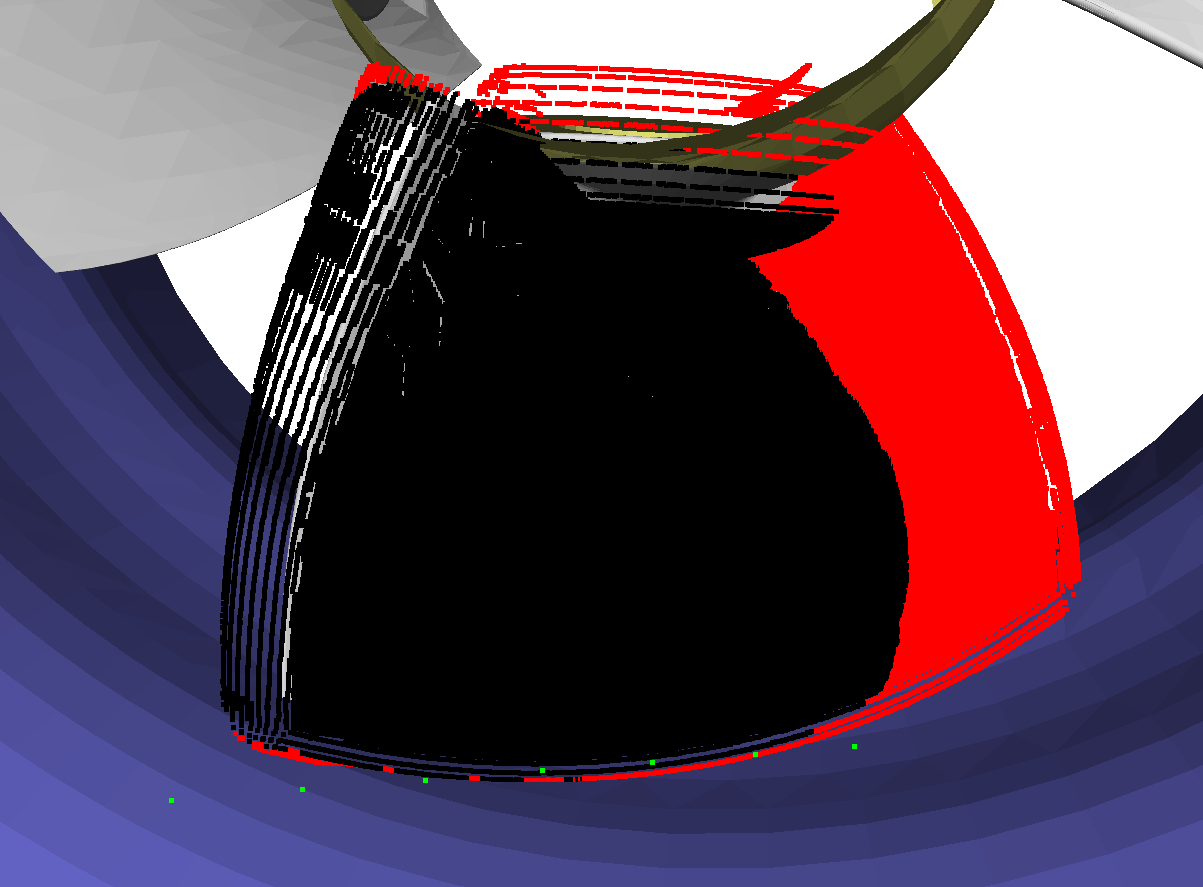
\includegraphics[width=\columnwidth]{method/figs/simcomp1_5.png}
	\caption{Simulação de revestimento completo da pá, considerando as
	restrições mecânicas da base, ângulo $-15^o$ do rotor e $24^o$ da pá.}
	\label{fig::simcomp1_5}
\end{figure}

Quando aumentamos a tolerância de ângulo de revestimento
para $60^o$, obtemos a figura\ref{fig::simcomp1_3}. A figura mostra que foi
possível revestir toda a extremidade superior esquerda, salvo pontos de colisão
com o rotor. Entretanto, é importante a base ter o grau de liberdade em $y$ para
suprir eventuais problemas de modelagem.

\begin{figure}[!ht]
	\centering	
	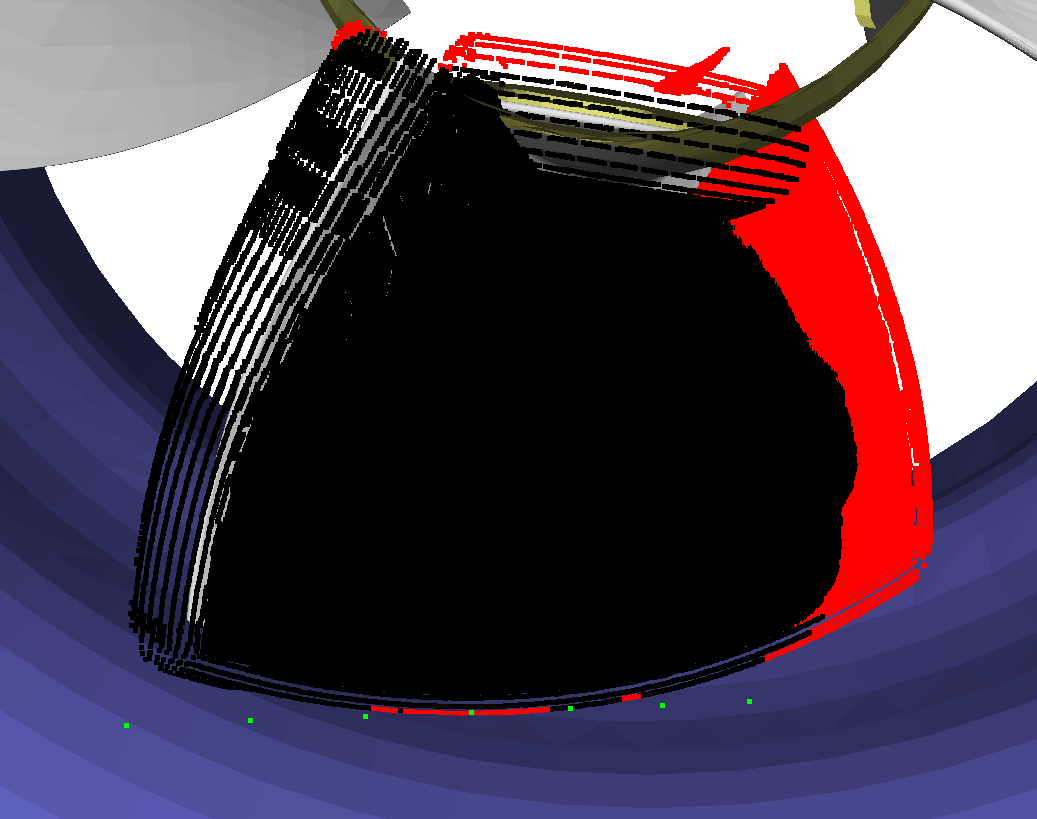
\includegraphics[width=\columnwidth]{method/figs/simcomp1_3.png}
	\caption{Simulação de revestimento completo da pá, considerando as
	restrições mecânicas da base, ângulo $0^o$ do rotor e $24^o$ da pá,
	tolerância de $60^o$ de revestimento.}
	\label{fig::simcomp1_3}
\end{figure}

Ao elevarmos a base $y+500 mm$, obtemos a figura~\ref{fig::simcomp1_6}. A figura
mostra que foi possível revestir toda a extremidade superior esquerda e, ainda,
alguns pontos na lateral direita que não haviam sido revestidos. É muito
provável que este grau de liberdade da base seja projetado, a fim de o projeto
não ficar dependente dos movimentos da turbina.

\begin{figure}[!ht]
	\centering	
	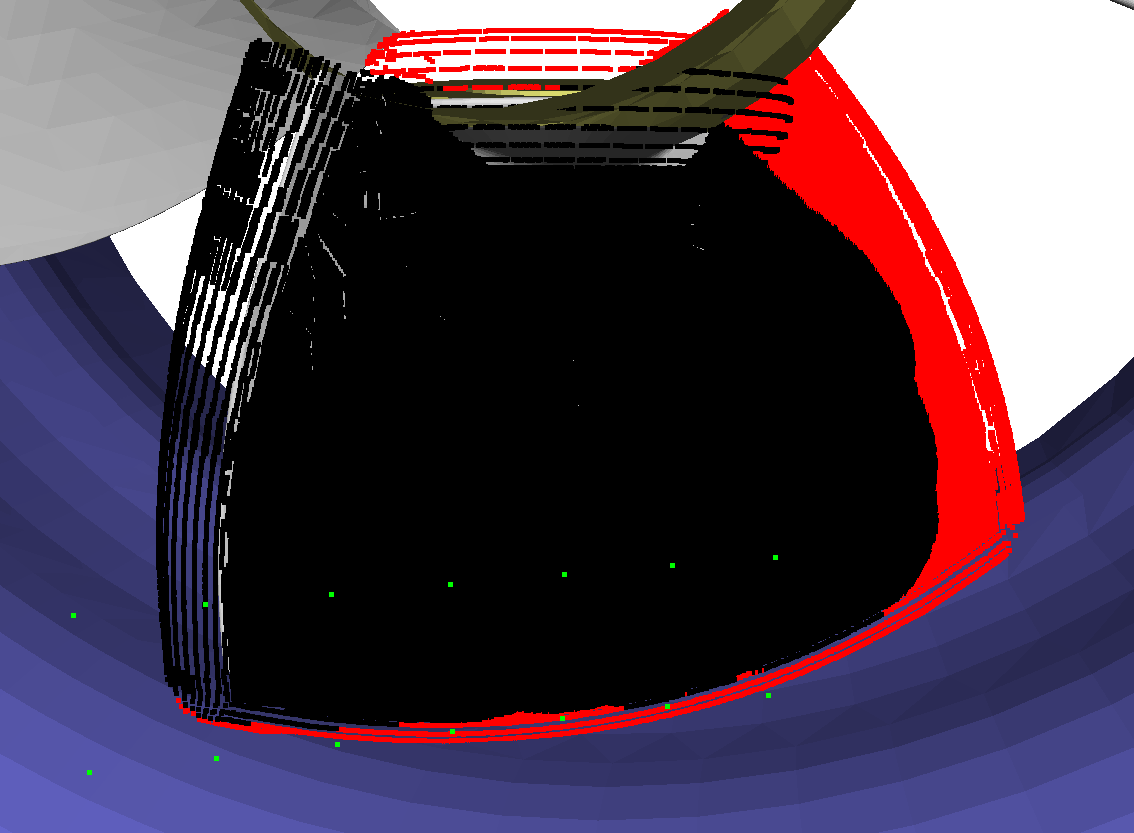
\includegraphics[width=\columnwidth]{method/figs/simcomp1_6.png}
	\caption{Simulação de revestimento completo da pá, considerando as
	restrições mecânicas da base, ângulo $0^o$ do rotor e $24^o$ da pá,
	$y+500 mm$.}
	\label{fig::simcomp1_6}
\end{figure}

\paragraph{Lateral direita}
Em relação à lateral direita da pá, a ideia imediata é rotar a turbina,
esperando que o lado direito se aproxime do robô. Outras possibilidades é
girar a pá em seu próprio eixo para $0^o$, em vez de $24^o$. As desvantagens de
cada solução se assemelham às discutidas previamente: rotar a turbina exige
transporte dos equipamentos à área de segurança, remontagem e recalibração;
girar a pá só é possível através do circuito hidráulico e talvez não seja
possível após início da operação.

A figura~\ref{fig::simcomp1_2} mostra a discretização completa da pá, nas
condições em que o rotor está $15^o$ e a pá $24^o$. Conforme o rotor é
girado no sentido anti-horário (positivo), embora o revestimento aumente na
lateral direita da pá, a lateral esquerda e as áreas inferiores começam a ser
prejudicadas. A extremidade superior direita continua sem ser revestida, como
esperado, vide subseção~\ref{superioresquerda}.

\begin{figure}[!ht]
	\centering	
	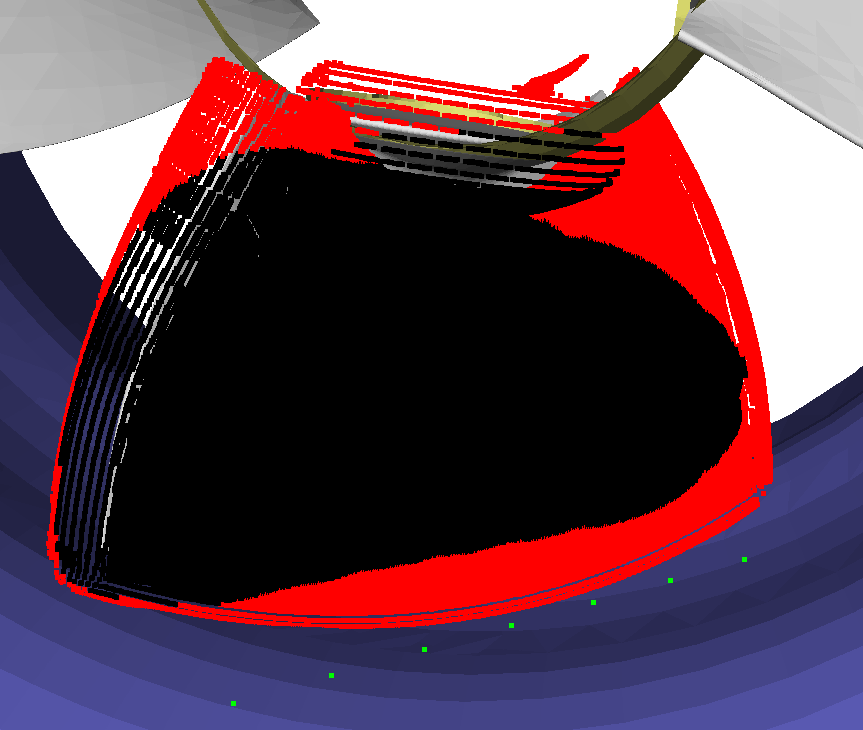
\includegraphics[width=\columnwidth]{method/figs/simcomp1_2.png}
	\caption{Simulação de revestimento completo da pá, considerando as
	restrições mecânicas da base, ângulo $15^o$ do rotor e $24^o$ da pá.}
	\label{fig::simcomp1_2}
\end{figure}

A figura~\ref{fig::simcomp1_4} mostra a discretização completa da pá, nas
condições em que o rotor está $0^o$ e a pá $0^o$. Conforme a pá é girada, o
revestimento aumenta na lateral direita e se mantém na lateral esquerda. Isso
ocorre, pois o robô se mantém longe do aro câmara no lado direito, já que o aro
ainda não está a $20^o$. Esta é a melhor posição para revestimento da pá,
situação aparente ao método empregado pela Rijeza. Entretanto, esta configuração
fornece pequeno espaçamento entre pás, estreitando a passagem do robô e, muito
provavelmente, não é possível alterar esse ângulo frequentemente já que exige
funcionamento do circuito hidráulico.

\begin{figure}[!ht]
	\centering	
	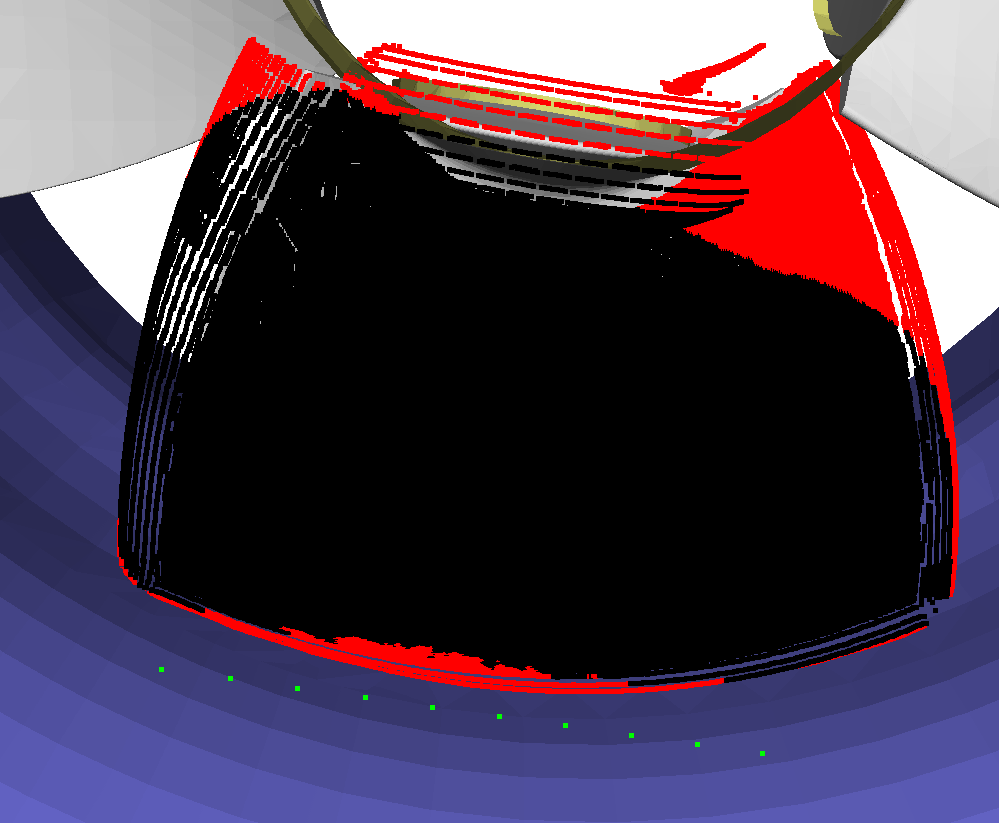
\includegraphics[width=\columnwidth]{method/figs/simcomp1_4.png}
	\caption{Simulação de revestimento completo da pá, considerando as
	restrições mecânicas da base, ângulo $0^o$ do rotor e $0^o$ da pá.}
	\label{fig::simcomp1_4}
\end{figure}

\paragraph{Extremidade superior direita}
A extremidade superior direita requer uma nova estratégia, pois todas as
outras falharam até então: rotacionar turbina, girar pá, elevar o robô no trilho
$y+500 mm$. Não há possibilidade, portanto, de realizar o revestimento a partir
do trilho 2 (posicionamento). A solução encontrada até o momento é rotar a
turbina $45^o$, manter a pá em $24^o$ e posicionar o robô entre as pás, no
trilho 1 (transporte). A desvantagem logística de rotar a turbina é comum às
soluções antigas, porém, esta configuração da turbina já estava prevista para
a entrada do robô no lado do distribuidor.

A figura~\ref{fig::simcomp1_7} mostra a discretização completa da pá, nas
condições em que o rotor está $45^o$ e a pá $24^o$. O robô se encontra
com sua base nas posições destacadas em verde. Como podemos observar, nesta
configuração (robô no trilho 1), é possível revestir a extremidade
superior direita. A fim de melhor aproveitamento logístico da
operação, esta operação deve ser realizada antes da entrada completa
do robô no lado do distribuidor.

\begin{figure}[!ht]
	\centering	
	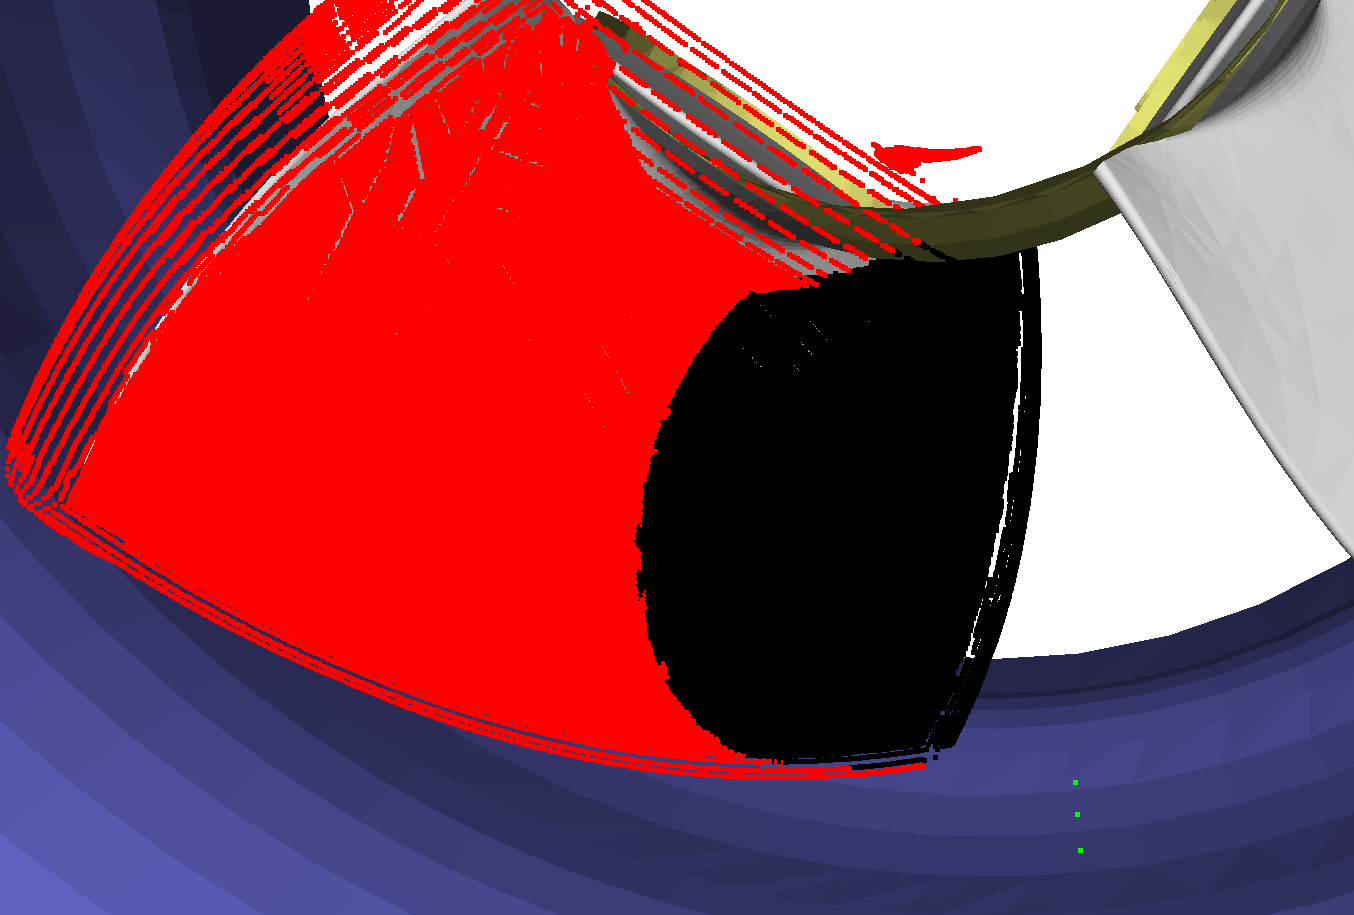
\includegraphics[width=\columnwidth]{method/figs/simcomp1_7.png}
	\caption{Simulação de revestimento completo da pá, considerando as
	restrições mecânicas da base, ângulo $45^o$ do rotor e $24^o$ da pá, robô
	entre as pás.}
	\label{fig::simcomp1_7}
\end{figure}

\paragraph{Conclusão da simulação completa}

A simulação completa da pá mostrou diversas estratégias para o revestimento da
pá, considerando as restrições mecânicas do trilho, o ambiente modelado da
turbina, e as diversas variáveis do processo de revestimento.

A partir dos resultados das simulações, podemos concluir que é possível realizar
o revestimento completo da pá, inclusive das áreas de mais difícil acesso, como
as extremidades. O revestimento completo, no entanto, requer uma extensa
logística de operação. Para cada face da pá, o robô deverá executar o
procedimento tanto no trilho de posicionamento (trilho 2), quanto no trilho de
transporte (trilho 1), a fim de revestir a área mais complexa, extremidade
superior direita. 